%
\chapter{Results of 1d3v PIC Simulation}\label{sec:chapter_onedcomparison}
%
    An existing 1d3v Particle-in-Cell code \cite{Matyash07oxIII,Matyash07PIC,Bronold07b} is used to understand the fundamental physics in a ccrf discharge of low pressures of oxygen. The limits of the code with respect to a realistic description of the experiment will also be discussed, which can only be resolved with a two-dimensional simulation.
%
    \section{Low Pressure Discharge of Oxygen}
%
        The 1D PIC-MCC code is applied to oxygen plasmas. Cross-section data for collisions are used as presented before in~\autoref{sec:negiondynamics} and shown in~\autoref{fig:cross_sections}.\\
        The simulation model resembles a parallel plate rf discharge. The electrodes are placed at both ends of the domain, e.g.\@ $x=0$ and $x=N\ix{z}\cdot\Delta z\ix{0}$. Scaling parameters were chosen as $n\ix{e,0}=$\SI{5e9}{\per\cubic\centi\metre} and $T\ix{e,0}=$\SI{5}{\electronvolt}. This results in a Debye length $\lambda\ix{D,e}=\,$\SI{0.0234}{\centi\metre} and an electron plasma frequency $\omega\ix{p,e}=\,$\SI{3.98e9}{\hertz}. The size of a cell is $\Delta z\ix{0}=\,$\SI{0.0117}{\centi\metre}.\\
        The domain length was set to $N\ix{z}=426$ cells, which corresponds to \SI{5.0}{\centi\metre}. Experience has shown that too small simulation domains result in a too small plasma bulk~\cite{Matthias15}, contradicting experimental observations. In such a case, the discharge would be dominated by the space charge sheaths in front of the electrodes. Therefore, no sufficiently sized plasma can be established to investigate the important ion dynamics. Parameters chosen here guarantee sufficiently large bulk regions.\\
        The cathode is driven sinusoidal at a frequency of $\SI{13.56}{\mega\hertz}$ with a voltage amplitude of \SI{400}{\volt}. It is placed at $z=$\SI{5.0}{\centi\metre}. The proposed model from~\autoref{sec:surfaceeffects} for the injection of negative ions at a surface is implemented and used here. An injection efficiency of $\eta=\,$0.03.~\cite{Meichsner13} is used due to the lack of reliable data.\\
%%%%%%%%%%%%%%%%%%%%%%%
%%%%%%%% LEFT EVEN PAGE
        \pagebreak
        \begin{figure}[!h]
            \centering
			\includegraphics[width=0.8\textwidth]%
                {figures/results/1D/potential.png}
            \caption[Phase resolved 1D potential]{%
                Phase resolved potential. Dynamics of the potential %
                for $U\ix{rf}=$\SI{400}{\volt} during one rf cycle, with %
                the mean plasma potential $\Phi_{av}$.}
            \label{fig:pot1d}
        \end{figure}
				\vfill
        \begin{figure}[!h]
            \centering
			\includegraphics[width=0.8\textwidth]%
                {figures/results/1D/densities.png}
            \caption[1D density distribution]{%
                Density distribution of electrons, postive and %
                and negative ions. The density of negative ions %
                produced by surface processes was separated.}
            \label{fig:dens1d}
        \end{figure}
		\pagebreak
%%%%%%%%%%%%%%%%%%%%%%%
%%%%%%%% RIGHT ODD PAGE				
        \begin{figure}[!h]
            \centering
			\includegraphics[width=0.8\textwidth]%
                {figures/results/1D/prs_ne_dens.png}
            \caption[Phase resolved 1D density profile]{%
                Phase resolved density of electrons, positive and negative %
				ions at \SI{2}{\pascal} and \SI{400}{\volt}. %
				Dashed and dotted lines are at different phases for all %
                species, respectively.}
            \label{fig:prsdens1d}
        \end{figure}
				\vfill
        \begin{figure}[!h]
            \centering
            \includegraphics[width=0.8\textwidth]%
				{figures/results/1D/densities_Omin.png}
            \caption[Negative ion density of surface and bulk processes]{%
                Density of negative ions that have been produced %
                in the bulk and at the surface --- subscript (b) and (s) respectively.}
            \label{fig:denscompare1d}
        \end{figure}
				\pagebreak
%
        Initially, all particles are randomly distributed across the whole domain. This includes the same amount of electrons and ions. The initialisation of a plasma bulk reduces the start-up in comparison to the initialisation of only a small number of free electrons and subsequent build-up of the rf plasma. The neutral gas is treated with $n\ix{n}=const.$ as an inexhaustible reservoir with fixed temperature $T=\SI{300}{\kelvin}$. The neutral pressure was chosen between 2--$\SI{10}{\pascal}$.\\
        Potential, ion and electron densities are shown in~\autoref{fig:pot1d} and~\autoref{fig:dens1d}. The potential is shown for different phases of the rf pulse. Also, the time-averaged plasma potential $\Phi\ix{av}$ is presented. Though the plasma potential is dominated by the driver on a shorter time scale, e.g\@ $\varphi=\pi/2,\dots$ the mean value rests at $\Phi=0$ at the electrodes and becomes $\Phi\approx\unit[200]{V}=U\ix{rf}/2$ in the bulk. The corresponding phase-resolved density distributions at the anode of electrons, negative and positive positive ions is shown next to it. One can easily see that only the electrons follow the externally applied electric field. The modulation of their density distribution is namely the oscillation of the space charge sheath, because both ion species remain stationary throughout the rf cycle.\\
        Figure~\ref{fig:dens1d} underlines the findings from~\autoref{fig:pot1d}. The charged species form a well developed plasma bulk of approximately \SI{3.5}{\centi\metre} length. Plasma sheaths on both sides are equally spaced with \SI{0.75}{\centi\meter}$\,\sim\,32\cdot\lambda\ix{D,e}$. They build up due to the potential drop between plasma bulk and electrodes. Because of the results from~\autoref{equ:langmuirpot} by Langmuir we know that the sheaths potential is a function of the unperturbed ion plasma current, or vice versa. Hence, the sheaths thickness establishes self consistently to satisfy current continuity $j\ix{e}=j\ix{i}$ at the boundaries. One also finds the electron density to decay much faster towards the walls in comparison the positive and negative ions. This is in agreement with the one-dimensional approximations from~\autoref{equ:ionandelectrondens}, where electron numbers decrease exponentially and the ion density only descends to the power of $-1/2$. Additionally, the potential drop between bulk and electrodes is equal on both sides, even when only one electrode is driven. It builds up self-consistently due to the afore-mentioned different ion and electron dynamics.\\
        In~\autoref{fig:dens1d} one can see that the sum of negative ion and electron density equals the positive ion density in the bulk due to the quasi-neutrality constraint. Towards the electrodes the plasma space charge separation establish and sheaths form as discussed before  in~\autoref{sec:sheathphysics}.The density of negative ions produced at the surface $O^{-}{(s)}$ increases towards the cathode. This is due to their production at the electrode.\\
        A comparison between the density of negative oxygen ions produced on the surface and plasma bulk is displayed in~\autoref{fig:denscompare1d}. The arrow marks a little density peak of $O^{-}_{(s)}$, which was highlighted before in~\autoref{fig:dens1d}. This structure in the $O^{-}_{(s)}$ density is a result of the deceleration of fast particles in the bulk by energy loss collisions. They are then reflected eventually at the sheath edges because of the potential barrier at the boundary.\\
%        
        \vspace*{-0.6cm}
        \begin{wrapfigure}[21]{r}{0.45\textwidth}
            \centering
            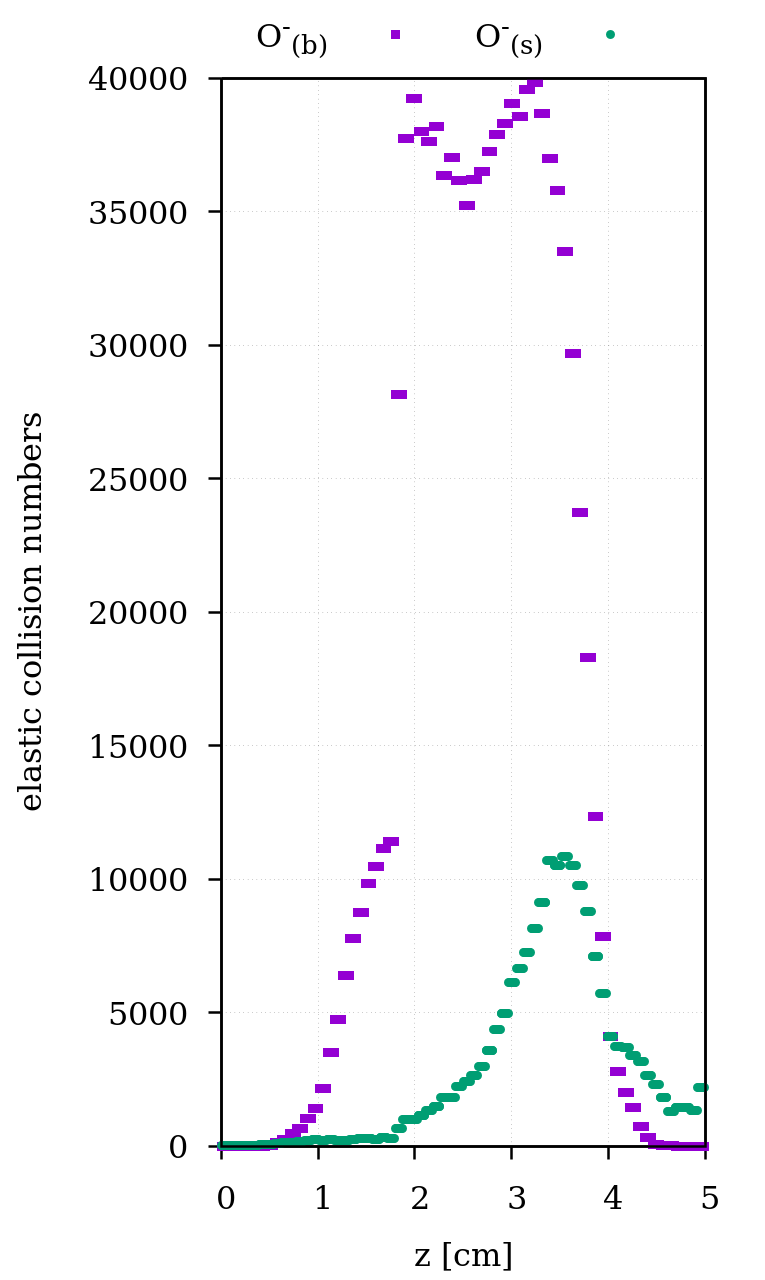
\includegraphics[width=0.42\textwidth]{figures/results/1D/elastcoll.png}
            \caption[Elastic collisions for surface and bulk anions]{%
                Elastic collisions of surface and bulk anions.}
            \label{fig:elastcoll1d}
        \end{wrapfigure}
%        
         The total number of collisions with neutral gas molecules for negative ions from the bulk and surface is shown in~\autoref{fig:elastcoll1d}. They include elastic scattering and charge exchange processes. As expected, most collisions happen in the bulk, but also some occur in the sheath at \SI{5}{cm}. Obviously the sheath is collisional. The collisions of energetic $O^{-}$ with low energy $O_{2}$ molecules at room temperature leads to a loss of kinetic energy. This is due to either elastic scattering or charge exchange processes, where the anion becomes cold when colliding with a molecule.\\
        Because I am interested in the dynamics of the plasma the energy distribution functions of the charged species are of particular interest, especially those of the surface generated $O^{-}$ ions. The next part is therefore devoted to the discussion of the particles EDF and the corresponding behaviour.
%        
    \section{Energy Distribution Functions and Anion Dynamics}
%
			The EDFs of both ion species have large particle counts at low energy values, distributed over the plasma bulk at the centre of the discharge. The corresponding kinetic temperatures for the majority of positive and negative ions are rather low, e.g\@ between $\tenpo{3}$K to $\tenpo{4}$K. This `cold core' expands from 50 to 370$\,\lambda\ix{D,e}$ and \SIrange{-5}{+5}{\electronvolt} respectively. The high energy part in the distribution function of $O^{+}_{2}$ between 0 -- 50$\,\lambda\ix{D,e}$, and 370 -- 426$\,\lambda\ix{D,e}$ is a result of the acceleration in the sheath by the potential drop of  $\approx\unit[200]{V}\,$. The low energy part of the distribution establishes through energy loss collisions and bulk ionisation processes with slow exit velocities.\\
        There are subtle structures in the positive ion EDF between electrodes and bulk below the higher energy distribution tail. One can count 7 to 8 of such characteristic peaks on both sides. This is likely the number of rf cycles an ion stays in the plasma sheath. Assuming the ion energy is approximately \SI{50}{\electronvolt} upon entering the sheath, an its thickness roughly \SI{0.75}{\centi\meter}, the transit time of the incident particle is $\approx\,$\SI{8.3} times the duration of a full radio frequency cycle. It is de-/accelerated inside the sheath, oscillating with the phase of the external electric field. Therefore, ions can gain up to 8 times the energy from the electric field in one RF cycle while passing through the sheath and flying towards the electrode. They are eventually reflected and likewise accelerated again in the opposite direction.\\
        The dynamics of the negatively charged electrons in the sheaths is very well highlighted in~\autoref{fig:edf_ex}. One can see the acceleration between 0--50$\,\lambda\ix{D,e}$, which yields energies of up to \SI{100}{\electronvolt}. The higher energy portion of the electrons from the anode traverses the bulk and is decelerated in the opposing sheath and vice versa. Also, the electron EDF has a low energy peak in the bulk between \SIrange{-50}{50}{\electronvolt}, whose numbers quickly decay to higher values due to energy loss collisions.\\
        In~\autoref{fig:edf_snix} the energy distribution of negative ions produced in the plasma bulk is shown. The form of electron and negative bulk ion EDF is similar in a sense that both show a low energy peak across the bulk length between 50 and 370$\,\lambda\ix{D,e}$. In contrast, fast electrons from the anode reach the cathode with a kinetic energy $E\ix{kin}>0$, as seen in~\autoref{fig:edf_ex}, whereas the negative ion distribution does not have this feature. Their distribution functions shows the intrinsic de-/acceleration in the sheaths of this symmetric discharge. Anions from the bulk never gain a kinetic energy large enough to pass the potential barrier at the electrodes. They are reflected at the boundary/in the sheath and eventually make it across the bulk to be reflected again.\\
        The distribution function of anions produced at the surface shows the acceleration by the potential drop in the plasma sheath, which yields kinetic energies up to \SI{120}{\electronvolt}. The corresponding peak can be found between 370 and 426$\,\lambda\ix{D,e}$ in~\autoref{fig:edf_snix}. There is also a peak at \SI{-50}/\SI{50}{\electronvolt} between 50 and 370$\,\lambda\ix{D,e}$. This is the result of fast particles being decelerated in the plasma bulk. They are reflected at the sheath edges because of their decreased kinetic energy, and therefore do not make it to the anode. Collisionless surface ions are reflected in the opposing, which is why there are similar structures to the ones discussed earlier between 0 and 50$\,\lambda\ix{D,e}$.\\
%%%%%%%%%%%%%%%%%%%%%%%
%%%%%%%% LEFT EVEN PAGE
%%%%%%%% ION AND NION
		\pagebreak
        \begin{figure}[!h]
            \centering
            \includegraphics[width=0.8\textwidth]%
				{figures/results/1D/ix_edf.png}
            \caption[Ion EDF in 1D]{%
                Logartihmic spatial-energetically %
				resolved EDF of postive ions from a discharge at %
				\SI{5}{\pascal} and \SI{400}{\volt}.}
			\label{fig:edf_ix}
        \end{figure}
				\vfill
        \begin{figure}[!h]
            \centering
        	\includegraphics[width=0.8\textwidth]%
				{figures/results/1D/nix_edf2.png}
            \caption[Negative ion EDF in 1D]{%
                Logarithmic spatial-energetically resolved EDF of negative %
                ions from a discharge at \SI{2}{\pascal} %
                and \SI{400}{\volt}.}
            \label{fig:edf_nix}
        \end{figure}
		\pagebreak
%%%%%%%%%%%%%%%%%%%%%%%
%%%%%%%% RIGHT ODD PAGE
%%%%%%%% EL AND SNION
        \begin{figure}[!h]
            \centering
            \includegraphics[width=0.8\textwidth]%
				{figures/results/1D/ex_edf.png}
            \caption[Electron EDF in 1D]{%
            	Logarithmic spatial-energetically resolved EDF of electrons %
            	from a discharge at \SI{2}{\pascal} and \SI{400}{\volt}.}
			\label{fig:edf_ex}
        \end{figure}
				\vfill
				\begin{figure}[!h]
            \centering
            \includegraphics[width=0.8\textwidth]%
					{figures/results/1D/snix_edf.png}
            \caption[Surface produced anion EDF in 1D]{%
                Logarithmic spatial-energetically resolved EDF %
                negative ions produced on the surface from %
		    	a discharge at \SI{2}{\pascal} and \SI{400}{\volt}.}
            \label{fig:edf_snix}
        \end{figure}
				\pagebreak
%                
        The surface anion EDF slightly increases towards the cathode. This is due to the asymmetric secondary ion emission, because we only considered the production of negative ions at the cathode. Additionally, there are also peaks similar to the one found for positive ions in the lower energy part of the EDF in front of the cathode. A closer look at this can be found in~\autoref{fig:snix_prs}.\\
        The~\autoref{fig:snixsurf} shows the high energy peak of the previously discussed surface anion distribution function. This structure decays with the mean free path of the negative ions. For example, the $O^{-}$ loses energy or it is lost by detachment at $O_{2}$ and recombination with $O^{+}_{2}$. This also creates the density peak in front of the cathode in~\autoref{fig:denscompare1d}. Negative ions from surfaces may become cold through energy loss collisions, which is why they eventually remain in the bulk.\\
        The subtle structure in the cathode sheath region of the surface anion EDF builds up due to the low transit time of a slow particle through the space charge area. Therefore the phase-resolved distribution function of the negative surface ions is shown in~\autoref{fig:snix_prs}. The modulation of the electrodes and sheaths potential causes de-/acceleration of the slow particles entering at approximately \SI{50}{ev}. They need \SI{4.32e-7}{\second} to travel through a sheath of thickness \SI{0.75}{\centi\meter} the given kinetic energy. It stays for roughly 5--6 rf cycles inside the sheath. This produces the same additional peak structures as for positive ions. In the phase-resolved EDF we can see anion density peaks moving according to the phase of the rf signal. Between five and six peaks are visible at a given moment in the excitation, which supports the findings from before. The ions enter the sheath easier when the voltage is positive during $\varphi\le\pi$. Afterwards they are accelerated away from the sheath at $\pi<\varphi\le2\pi$. The anions/ions oscillate back and forth. Their kinetic energy is transferred into potential energy in the sheath and vice versa.\\
        The particle numbers in the EDF of surface ions are at least one order of magnitude smaller than those of the bulk ions. This is due to the low surface production of an efficiency $\eta=\,$0.03~\cite{Meichsner13} at the cathode and low pressures of \SI{2}{\pascal}, which favours the production of anions in the plasma volume.\\
        Figure (\ref{fig:compare_ied}) confirms, in comparison with the experimental results from~\autoref{fig:expresults}, that negative ions produced at the surface may lead to the measured high-energy peak. The energy distribution function of the simulation has additional low energy peaks at $<\unit[100]{eV}$, too. They are created due to the energy loss by collisions and the intrinsic symmetry of the sheaths. This peak structure was also found and discussed for~\autoref{fig:snixsurf}.\\
        In the experiment all high-energy anions are detected by a mass-spectrometer and thereby removed from the discharge. In this simulation however, the collection of the energy distribution function does not perturb the results in any way.
%%%%%%%%%%%%%%%%%%%%%%%
%%%%%%%% LEFT EVEN PAGE
%%%%%%%% SNION CLOSE UP SURF
				\pagebreak
        \begin{figure}[!h]
            \centering
            \includegraphics[width=0.8\textwidth]%
				{figures/results/1D/snix_close_edf.png}
            \caption[Surface anion EDF close up]{%
				Same EDF as shown in~\autoref{fig:edf_snix}. %
                Close up the structures in the cathode sec:sheathphysics.}
            \label{fig:snixclose}
        \end{figure}
		\vfill
		\begin{figure}[!h]
        	\centering
        	\includegraphics[width=0.9\textwidth]%
					{figures/results/1D/snix_surface_edf.png}
            \caption[Negative ion EDF surface plot]{%
    			EDF as in~\autoref{fig:edf_snix} as a surface plot. %
    			One can see the energy peak at around\SI{-100}{\electronvolt} %
    			decaying over the length of the bulk.}
            \label{fig:snixsurf}
        \end{figure}
				\pagebreak
%%%%%%%%%%%%%%%%%%%%%%%
%%%%%%%% RIGHT ODD PAGE
%%%%%%%% PHASE RESOLVED
        \begin{figure}[!h]
            \centering
            \includegraphics[width=1.0\textwidth]%
				{figures/results/1D/snix_allpi_edf2.png}
            \caption[Phase resolved structures in the EDF of surface ions]{%
                Phase resolved surface anion energy distribution %
                functions in front of the cathode.}
            \label{fig:snix_prs}
        \end{figure}
        
        We have now thoroughly investigated the formation and dynamics of surface produced secondary anions in a 1d3v PIC simulation. It was found that surface ions have a significant impact on the energy distribution function of $O^{-}$. However, it was not seen that fast anions created at the surface of the cathode impinge onto the anode. This is due to the intrinsic acceleration in the potential of the sheath, and therefore deceleration in the opposing space charge. One can already tell this from the averaged potential in~\autoref{fig:pot1d}. A key element to the solution of this problem id the asymmetry of the driven discharge with a self bias voltage. This leads to a stronger acceleration at the cathode than retardation at the anode, and hence to the impact onto the electrode.\\
        The self consistent adjustment of plasma electron and ion current between volume and sheath makes it impossible to implement asymmetry in an one-dimensional simulations. The physics of bulk and sheath are governing the establishment of space charges, as well as the corresponding potential drops towards walls.
%
        \begin{figure}[!h]
            \centering
            \includegraphics[width=0.8\textwidth]%
				{figures/SFB/power_energy_cuts.png}
            \caption[EDF results from 1D at the anode]{%
                Energy distribution of negative ions $O^-$. Simulation result taken %
                at the anode sheath edge at different rf powers at $\unit[5]{Pa}$.}
            \label{fig:compare_ied}
        \end{figure}
%        
        Like it was discussed by Bronold and Matyash et al. in~\cite{Bronold07b}, the key argument for a one-dimensional simulation is the large electrode diameter in comparison to the electrode gap. Here it is said that the plasma properties are not affected, or at least the influence is considered negligible, by the boundaries of the electrodes. Along the axial centre of the discharge the plasma `does not see' the edge of the electrodes and therefore no asymmetry effects should take place~\cite{Matthias15}.\\
        From the results found by~\cite{Scheuer15} we know that fast ions can impinge onto the anode. Hence one needs a better model to describe the relevant physics of the experiment. A step towards this solution is the introduction of a two-dimension PIC simulation in which asymmetry effects such as self bias are implemented. The next chapter is devoted to that topic.
